\chapter{Numerical Solutions to Initial Value Problems}
Differential equations have numerous applications to describe dynamics from physics to biology to economics.\\

Initial value problems are subset of \addtoindex{Ordinary Differential Equation} (\addtoindex{ODE}'s) with the form
\begin{equation}
\label{ODE}
y^{'}=f(x)
\end{equation}
$f$ is a function.  The general solution to (\ref{ODE})
is
\[
y=\int f(x)dx +c,
\]
 containing an arbitrary constant $c$.  In order to determine the solution uniquely it is necessary to impose an initial condition,
\begin{equation}
\label{Initial condition}
y(x_0)=y_0.
\end{equation}

\begin{example}
\textbf{Simple Example}\\
The differential equation describes the rate of change of an oscillating input. 
The general solution of the equation
\begin{equation}\label{ODE_sine} y^{'}=\sin(x) \end{equation}
is, 
\[ y=-\cos(x)+c, \]
with the initial condition,
\[y(0)=2,\]
then it is easy to find $c=2$.\\
Thus the desired solution is,
\[ y=2-\cos(x). \]
\end{example}

The more general \addtoindex{Ordinary Differential Equation} is of the form
\begin{equation}
\label{general ODE}
y^{'}=f(x,y),
\end{equation}
is approached in a similar fashion.\\
Let us consider
\[ y^{'} = a(x)y(x)+b(x),\]
The given functions $a(x)$ and $b(x)$ are assumed continuous for this equation
\[f(x,z)=a(x)z(x)+b(x), \] 
and the general solution can be found using the method of integrating factors.
\begin{example}
\textbf{General Example}\\
Differential equations of the form
\begin{equation}
\label{eqn A}
y^{'}(x)=\lambda y(x) +b(x), \ \ \ \ x \geq x_0,
\end{equation}
where  $\lambda$ is a given constant and $b(x)$ is a continuous integrable function has a unique analytic. Multiplying the equation (\ref{eqn A}) by the 
integrating factor $e^{-\lambda x}$, we can reformulate
\[\frac{d(e^{-\lambda x}y(x))}{dx}=e^{-\lambda x}b(x). \]
Integrating both sides from $x_0$ to $x$ we obtain
\[(e^{-\lambda x}y(x))=c+\int_{x_0}^{x}e^{-\lambda t}b(t)dt, \]
so the general solution is
\[y(x)=ce^{\lambda x}+\int_{x_0}^{x}e^{\lambda(x-t)}b(t)dt, \]
with $c$ an arbitrary constant
\[ c=e^{-\lambda x_0} y(x_0). \]
\end{example}

For a great number of Initial Value Problems there is no known exact (analytic) solution as the equations are non-linear, for example
$y^{'} = e^{xy^4}$, or discontinuous or stochastic. There for a numerical method is used to approximate the solution.  

\section{Numerical approximation of Differentiation}
\subsection{Derivation of Forward Euler for one step}
The left hand side of a initial value problem $\frac{df}{dx}$ can be approximated by  \textbf{Taylors theorem} expand about a point $x_0$ giving:
\begin{equation}f(x_1) = f(x_0)+(x_1-x_0)f^{'}(x_0) + \tau, \end{equation}
where $\tau$ is the truncation error,
\begin{equation}h\tau = \frac{(x_1-x_0)^2}{2!}f^{''}(\xi), \ \ \ \ \ \ \xi \in [x_0,x_1]. \end{equation}
Rearranging and letting $h=x_1-x_0$ the equation becomes
\[f^{'}(x_0)=\frac{f(x_1)-f(x_0)}{h}-\frac{h}{2}f^{''}(\xi). \]
Term $-\frac{h}{2}f^{''}(\xi)$ is known as the local truncation error.
The forward Euler method can also be derived using a variation on the Lagrange interpolation formula
called the divided difference. \\
Any function $f(x)$ can be approximated by a polynomial of degree $P_n(x)$ and an error term,
\begin{eqnarray*}
f(x)&=&P_n(x) + error,\\
&=&f(x_0)+f[x_0,x_1](x-x_0)+f[x_0,x_1,x_2](x-x_0)(x-x_1),\\
& &+...+f[x_0,...,x_n]\Pi_{i=0}^{n-1}(x-x_i)+error,
\end{eqnarray*}
where 
\[f[x_0,x_1] = \frac{f(x_1)-f(x_0)}{x_1-x_0},\]
\[f[x_0,x_1,x_2] = \frac{f[x_1,x_2]-f[x_0,x_1]}{x_2-x_0},\]
\[f[x_0,x_1,..,x_n] = \frac{f[x_1,x_2,...,x_n]-f[x_0,x_1,...,x_{n-1}]}{x_n-x_0},\]
Differentiating $P_n(x)$
\begin{eqnarray*}
P_n^{'}(x)=f[x_0,x_1]+f[x_0,x_1,x_2]\{(x-x_0)+(x-x_1)\}, \\
+...+f[x_0,...,x_n]\sum_{i=0}^{n-1}\frac{(x-x_0)...(x-x_{n-1})}{(x-x_i)},\end{eqnarray*}
and the error becomes
\[
error= (x-x_0)...(x-x_n)\frac{f^{n+1}(\xi)}{(n+1)!}.
\]
Applying this to define our first derivative, we have
\[
f^{'}(x)=f[x_0,x_1] = \frac{f(x_1)-f(x_0)}{x_1-x_0},\]
this leads us other formulas for computing the derivatives
\[ f^{'}(x) = \frac{f(x_1)-f(x_0)}{x_1-x_0}+O(h), \ \ \mbox{  Euler,  }\]
\[ f^{'}(x) = \frac{f(x_1)-f(x_{-1})}{x_1-x_{-1}}+O(h^2), \ \ \mbox{    Central.  }\]
Using the same method we can get out computational estimates for the 2nd 
derivative
\[f^{''}(x_0)=\frac{f_{2}-2f_1+f_0}{h^2}+O(h^2),\]
\[f^{''}(x_0)=\frac{f_{1}-2f_0+f_{-1}}{h^2}+O(h^2), \ \ \mbox{   central.}\]
\begin{example} To numerically solve the first order \addtoindex{Ordinary Differential Equation} (\ref{general ODE})
\[ y^{'} = f(x,y), \]
\[a\leq x \leq b, \]
the derivative $y{'}$ is approximated by \[\frac{w_{i+1}-w_{i}}{x_{i+1}-x_{i}}=\frac{w_{i+1}-w_{i}}{h},\]
where $w_i$ is the numerical approximation of $y$ at $x_i$.
The Differential Equation is converted to a discrete difference equation with steps of size $h$, 
\[\frac{w_{i+1}-w_i}{h}=f(x_i,w). \]
Rearranging the difference equation gives the equation 
\[w_{i+1}=w_i+hf(x_i,w), \]
which can be used to approximate the solution at $w_{i+1}$ given information about $y$ at point $x_i$.
\end{example}

\subsubsection{Simple example ODE $y'=\sin(x)$}

\begin{example} Applying the Euler formula to the first order equation with an oscillating input
(\ref{ODE_sine})
\[ y^{'} = \sin(x), \]
\[0\leq x \leq 10. \]
The equation can be approximated using the forward Euler as 
\[\frac{w_{i+1}-w_i}{h}=\sin(x_i). \]
Rearranging the equation gives the discrete difference equation with the unknowns on the left and the know values of the right
\[w_{i+1}=w_i+h\sin(x_i). \]
The Python code bellow implements this difference equation. The output of the code is shown in Figure \ref{Sine wave ODE}.


\begin{lstlisting}[language=Python, caption=Python Numerical and Analytical Solution of Eqn \ref{ODE_sine} ]
# Numerical solution of a Cosine differential equation
import numpy as np
import math 
import matplotlib.pyplot as plt

h=0.01
a=0
b=10

N=int(b-a/h)
w=np.zeros(N)
x=np.zeros(N)
Analytic_Solution=np.zeros(N)

# Initial Conditions
w[0]=1.0
x[0]=0
Analytic_Solution[0]=1.0
for i in range (1,N):
    w[i]=w[i-1]+h*math.sin(x[i-1])
    x[i]=x[i-1]+h
    Analytic_Solution[i]=2.0-math.cos(x[i])

fig = plt.figure(figsize=(8,4))

# --- left hand plot
ax = fig.add_subplot(1,3,1)
plt.plot(x,w,color='red')
#ax.legend(loc='best')
plt.title('Numerical Solution')

# --- right hand plot
ax = fig.add_subplot(1,3,2)
plt.plot(x,Analytic_Solution,color='blue')
plt.title('Analytic Solution')

#ax.legend(loc='best')
ax = fig.add_subplot(1,3,3)
plt.plot(x,Analytic_Solution-w,color='blue')
plt.title('Error')

# --- title, explanatory text and save
fig.suptitle('Sine Solution', fontsize=20)
plt.tight_layout()
plt.subplots_adjust(top=0.85)
\end{lstlisting}

\end{example}

\begin{figure}[h]
\centering
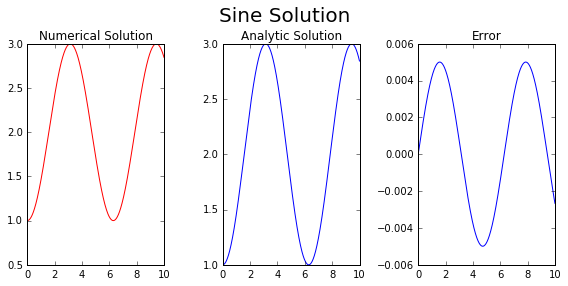
\includegraphics[scale=0.5]{sine_wave}
\caption{Python output: Numerical (left), Analytic (middle) and error(right) for $y'=\sin(x)$ Equation \ref{ODE_sine} with h=0.01}
\label{Sine wave ODE}
\end{figure}

\subsubsection{Simple example problem population growth $y^{'}=\ve y. $ }

\begin{example}
Simple population growth can be describe as a first order differential equation of the form: \begin{equation}\label{ODE_Growth} y^{'}=\ve y. \end{equation}
This has an exact solution of 
\[ y=Ce^{\ve x}. \]
Given the initial condition of  condition
\[y(0)=1\]
and a rate of change of
\[ \ve=0.5\]
the analytic solution is
\[ y=e^{0.5x}.\]

\end{example}

\begin{example} Applying the Euler formula to the first order equation
(\ref{ODE_Growth})
\[ y^{'} = 0.5y \]
is approximated by
\[\frac{w_{i+1}-w_i}{h}=0.5w_i. \]
Rearranging the equation gives the difference equation
\[w_{i+1}=w_i+h(0.5w_i). \]
The Python code below and the output is plotted in Figure \ref{GROWTH ODE Figure}.

\begin{lstlisting}[language=Python, caption=Python Numerical and Analytical Solution of Eqn \ref{ODE_Growth} ]
# Numerical solution of a differential equation
import numpy as np
import math 
import matplotlib.pyplot as plt

h=0.01
tau=0.5
a=0
b=10

N=int((b-a)/h)
w=np.zeros(N)
x=np.zeros(N)
Analytic_Solution=np.zeros(N)

Numerical_Solution[0]=1
x[0]=0
w[0]=1

for i in range (1,N):
    w[i]=w[i-1]+dx*(tau)*w[i-1]
    x[i]=x[i-1]+dx
    Analytic_Solution[i]=math.exp(tau*x[i])


fig = plt.figure(figsize=(8,4))
# --- left hand plot
ax = fig.add_subplot(1,3,1)
plt.plot(x,w,color='red')
#ax.legend(loc='best')
plt.title('Numerical Solution')

# --- right hand plot
ax = fig.add_subplot(1,3,2)
plt.plot(x,Analytic_Solution,color='blue')
plt.title('Analytic Solution')

#ax.legend(loc='best')
ax = fig.add_subplot(1,3,3)
plt.plot(x,Analytic_Solution-Numerical_Solution,color='blue')
plt.title('Error')

# --- title, explanatory text and save
fig.suptitle('Exponential Growth Solution', fontsize=20)
plt.tight_layout()
plt.subplots_adjust(top=0.85)
\end{lstlisting}
\end{example}

\begin{figure}[H]
\centering
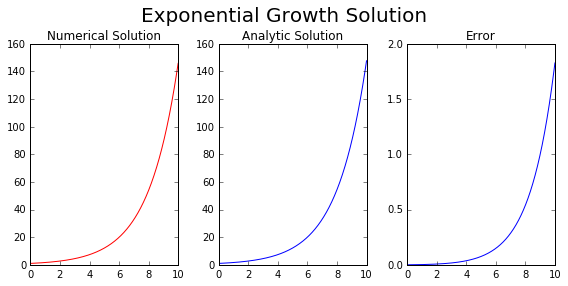
\includegraphics[scale=0.5]{ODE_Growth}
\caption{Python output: Numerical (left), Analytic (middle) and error(right) for $y^{'}=\ve y$  Eqn \ref{ODE_Growth} with h=0.01 and $\ve=0.5$}
\label{GROWTH ODE Figure}
\end{figure}

\subsubsection{Example of exponential growth with a wiggle}

\begin{example}
An extension of the exponential growth differential equation includes a sinusoidal component 
\begin{equation}\label{ODE_Growth_wiggle} y^{'}=\ve (y+y \sin(x)). \end{equation}
This complicates the exact solution but the numerical approach is more or less the same.
The difference equation is 
\[w_{i+1}=w_i+h(0.5w_i+w_i\sin(x_i)). \]
Figure \ref{GROWTH ODE WIGGLE} illustrates the numerical solution of the differential equation.

\begin{figure}[H]
\centering
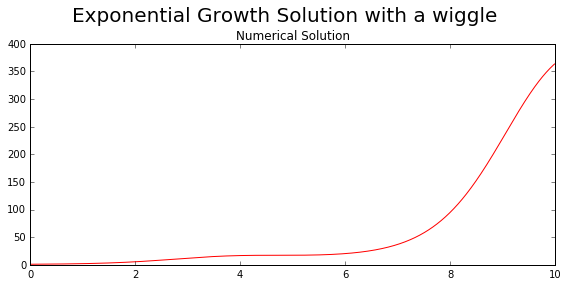
\includegraphics[scale=0.5]{ODE_Growth_with_a_wiggle}
\caption{Python output: Numerical solution for $y^{'}=\ve (y+y sin(x))$ Equation \ref{ODE_Growth_wiggle} with h=0.01 and $\ve=0.5$}
\label{GROWTH ODE WIGGLE}
\end{figure}

\end{example}

\subsection{Theorems about Ordinary Differential Equations}
\begin{definition}
A function $f(t,y)$ is said to satisfy a \textbf{\addtoindex{Lipschitz Condition}} in the variable $y$ on 
the set $D \subset R^2$ if a constant $L>0$ exist with the property that
\[|f(t,y_1)-f(t,y_2)| < L|y_1-y_2|, \]
whenever $(t,y_1),(t,y_2) \in D$.  The constant L is call the \addtoindex{Lipschitz Condition}
of $f$.
\end{definition}
\begin{definition}
A set $D\subset R^2$ is said to be convex if whenever $(t_1,y_1),(t_2,y_2)$ belong
to $D$ the point $((1-\lambda)t_1+\lambda t_2, (1-\lambda)y_1+\lambda y_2)$ also
belongs in $D$ for each $\lambda \in [0,1]$.
\end{definition}
\begin{theorem}
Suppose $f(t,y)$ is defined on a convex set $D \subset R^2$. If a constant
$L>0$ exists with
\[L\leq \left|\frac{\partial f(t,y)}{\partial y}\right|, \]
then $f$ satisfies a \addtoindex{Lipschitz Condition} an $D$ in the variable $y$ with
Lipschitz constant L.
\end{theorem}
\begin{theorem}
Suppose that
$D= \{(t,y) | a\leq t \leq b, -\infty <y < \infty \},$
and $f(t,y)$ is continuous on $D$ in the variable $y$ then the initial value
problem has a unique solution $y(t)$ for $a\leq t \leq b$.
\end{theorem}
\begin{definition}
The initial-value problem 
\[\frac{dy}{dt}=f(t,y), \ \ \ \ \  a\leq t \leq b,\]
with initial condition
\[y(a) = \alpha, \]
is said to be well posed if:
\begin{itemize}
\item
A unique solution $y(t)$ to the problem exists;
\item
For any $\varepsilon >0$ there exists a positive constant $k(\varepsilon)$
with the property that whenever $|\varepsilon_0| < \varepsilon$ and with
$|\delta(t)| \varepsilon$ on $[a,b]$ a unique solution $z(t)$ to the problem
\begin{equation} 
\label{perturbed}
\frac{dz}{dt}=f(t,z)+\delta(t), \ \ \  a\leq t \leq b, \end{equation}

\[z(a)=\alpha +\varepsilon_0, \]
exists with
\[ |z(t) - y(t) | < k(\varepsilon)\varepsilon. \]
The problem specified by (\ref{perturbed}) is called a perturbed problem associated
with the original problem.
\end{itemize}
It assumes the possibility of an error $\delta(\varepsilon)$ being introduced to
the statement of the differential equation as well as an error $\varepsilon_0$
being present in the initial condition.

\end{definition}
\begin{theorem}
Suppose $D= \{(t,y) | a\leq t \leq b, -\infty <y < \infty \}$.
If $f(t,y)$ is continuous and satisfies a \addtoindex{Lipschitz Condition} in the variable y on
the set $D$, then the initial value problem 
\[\frac{dy}{dt}=f(t,y), \ \ \  a\leq t \leq b,\]
with initial condition
\[y(a) = \alpha, \]
is well-posed.
\end{theorem}
\begin{example}
\[y^{'}(x)=-y(x)+1, \ \ \ \ 0\leq x \leq b, \ \ \ \ y(0)=1 \]
has the solution $y(x)=1$. The perturbed problem
\[z^{'}(x)=-z(x)+1, \ \ \ \ 0\leq x \leq b, \ \ \ \ z(0)=1+\va, \]
has the solution $z(x)=1+\va e^{-x}$ $x \leq 0$.\\
Thus 
\[y(x)-z(x)=-\va e^{-x} \]
\[|y(x)-z(x)|\leq |\va| \ \ \ \ x \geq 0 \]
Therefore the problem is said to be stable. This is illustrated in Figure \ref{Stable ODE}. 
\begin{figure}[H]
\centering
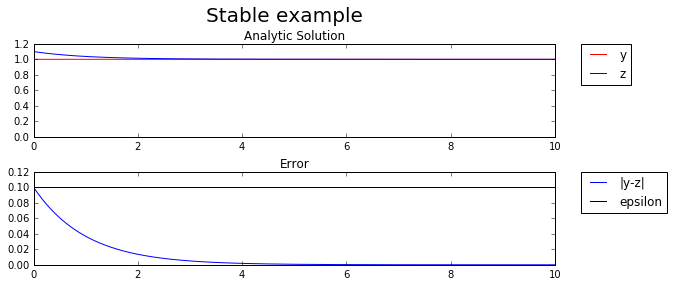
\includegraphics[scale=0.4]{Stable_example}
\caption{Python output: Illustrating Stability $y^{'}(x)=-y(x)+1$ with the initial condition $y(0)=1$ and $z^{'}(x)=-z(x)+1$ with the initial condition $z(0)=1+\va$, $\va=0.1$}
\label{Stable ODE}
\end{figure}

\end{example}

\section{One-Step Methods}
Dividing $[a,b]$ in to N subsections
such that we now have N+1 points of equal spacing $h=\frac{b-a}{N}$. This gives
the formula $t_i=a+ih$ for $i=0,1,...,N$.  
One-Step Methods for \addtoindex{Ordinary Differential Equation}'s only use one previous point to get
the approximation for the next point.  The initial condition gives $y(a=t_0)=\alpha$, this gives the starting point of our one step method.  The general formula
for One-step methods is 
\[ w_{i+1}=w_i+h\Phi(t_i,w_i,h), \] 
where $w_i$ is the approximated solution of the \addtoindex{Ordinary Differential Equation} at the point $t_i$
\[w_i\approx y_i.\]

\subsection{Euler's Method}
The simplest example of a one step method is Euler. The derivative is replaced
by the Euler approximation. The \addtoindex{Ordinary Differential Equation}
\[ \frac{dy}{dt}=f(t,y), \]
is discretised
\[\frac{y_i-y_{i-1}}{h}=f(t_{i-1},y_{i-1}) +T\]
T is the truncation error.\\
\begin{example}
Consider the Initial Value Problem
\[y^{'} = -\frac{y^2}{1+t}, \ \ \ a=0\leq t \leq b=0.5, \]
with the initial condition $y(0)=1$
the Euler approximation is
\[w_{i+1}=w_i -\frac{hw_i^2}{1+t_i}, \]
where $w_i$ is the approximation of $y$ at $t_i$.\\
Solving, let $t_i=ih$ where $h=0.05$, from the initial condition we have
$w_0=1$
at $i=0$ our method is 
\[w_1=w_0-\frac{0.05w^2_0}{1+t_0}=1-\frac{0.05}{1+0}=0.95 \]
and so forth, each approximation $w_i$ requiring the previous, thus creating a 
sequence starting at $w_0$ to $w_n$. The Table below show the numerical approximation for 10 steps.
\begin{center}
\begin{tabular}{ c| c |c }
  i& $t_i$& $w_i$\\
  \hline
 0 & $0$  & 1 \\  
 1 & $0.05$  & 0.95 \\  
 2 & $0.1$  & 0.90702381 \\  
 3 & $0.15$  & 0.86962871 \\  
 4 & $0.2$  & 0.8367481 \\  
 5 & $0.25$  & 0.80757529 \\  
 6 & $0.3$  & 0.78148818 \\  
 7 & $0.35$  & 0.7579988 \\  
 8 & $0.4$  & 0.73671872 \\  
 9 & $0.45$  & 0.71733463  
\end{tabular}
\end{center}
\end{example}

\begin{lemma}
\label{lemma 1}
For all $ x \geq 0.1$ and any positive m we have \[0\leq (1+x)^m \leq e^{mx}.\]
\end{lemma}

\begin{lemma}
\label{lemma 2}
If s and t are positive real numbers $\{a_i\}_{i=0}^{N}$ is a sequence satisfying $\displaystyle a_0 \geq \frac{-q}{s}$ and $a_{i+1} \leq (1+s)a_i +q $
then,
\[a_{i+1} \leq e^{(i+1)s}\left(a_0+\frac{q}{s}\right)-\frac{q}{s}. \] 
\end{lemma}
\begin{theorem}
\label{Euler bound}
Suppose $f$ is continuous and satisfies a \addtoindex{Lipschitz Condition} with constant
L on $D=\{(t,y)|a\leq t \leq b, -\infty < y < \infty \}$ and that a constant $M$
exists with the property that 
\[ |y^{''}(t)|\leq M. \]
Let $y(t)$ denote the unique solution of the \addtoindex{Initial Value Problem}
\[ y^{'}=f(t,y), \ \ \ a\leq t \leq b, \ \ \ y(a)=\alpha, \]
and $w_0,w_1,...,w_N$ be the approx generated by the Euler method for some
positive integer $N$.  Then for $i=0,1,...,N$
\[ |y(t_i)-w_i| \leq \frac{Mh}{2L}|e^{L(t_i-a)}-1|. \]
\end{theorem}
\begin{proof}
When $i=0$ the result is clearly true since $y(t_0)=w_0=\alpha$.
From Taylor we have,
\[y(t_{i+1})=y(t_i)+hf(t_i,y(t_i))+\frac{h^2}{2}y^{''}(\xi_i), \]
where $x_i \geq \xi_i \geq x_{i+1}$, and from this we get the Euler approximation
\[w_{i+1}=w_i + hf(t_i,w_i). \]
Consequently we have
\[y(t_{i+1})-w_{i+1}=y(t_i)-w_i+h[f(t_i,y(t_i))-f(t_i,w_i)]+\frac{h^2}{2}y^{''}(\xi_i), \]
and
\[|y(t_{i+1})-w_{i+1}|\leq |y(t_i)-w_i|+h|f(t_i,y(t_i))-f(t_i,w_i)|+\frac{h^2}{2}|y^{''}(\xi_i)|. \]
Since $f$ satisfies a \addtoindex{Lipschitz Condition} in the second variable with constant $L$
and $|y^{''}|\leq M$ we have
\[|y(t_{i+1})-w_{i+1}|\leq (1+hL)|y(t_i)-w_i|+\frac{h^2}{2}M. \]
Using Lemma \ref{lemma 1} and \ref{lemma 2} and letting $a_j=(y_j-w_j)$ for each
$j=0,..,N$ while $s=hL$ and $q=\frac{h^2M}{2}$ we see that
\[|y(t_{i+1}-w_{i+1}|\leq e^{(i+1)hL}(|y(t_0)-w_0|+\frac{h^2M}{2hL}) -\frac{h^2M}{2hL}. \]
Since $w_0-y_0=0$ and $(i+1)h=t_{i+1}-t_0=t_{i+1}-a$ we have
\[ |y(t_i)-w_i| \leq \frac{Mh}{2L}|e^{L(t_i-a)}-1|, \]
for each $i=0,1,..N-1$.
\end{proof}
\begin{example}
\[y^{'}=y-t^2+1, \ \ \ 0 \leq t \leq 2, \ \ \ y(0)=0.5, \]
the Euler approximation is
\[w_{i+1} = w_i + h(w_i-t_i^2+1) \]
choosing $h=0.2$, $t_i=0.2i$ and $w_0=0.5$. \\
$f(t,y)=y-t^2+1$
\[\frac{\partial f}{\partial y}=1 \]
so $L=1$. The exact solution is $y(t)=(t+1)^2-\frac{1}{2}e^t$ from this we have
\[y^{''}(t) = 2-0.5e^t, \]
\[|y^{''}(t)| \leq 0.5e^2-2, \ \ t\in[0,2].\]
Using the above inequality we have we have
\[|y_i-w_i| \leq \frac{h}{2}(0.5e^2-2)(e^{t_i}-1).\]
Figure \ref{UpperBound Figure} illustrates the upper bound of the error and the actual error.

\begin{figure}[H]
\centering
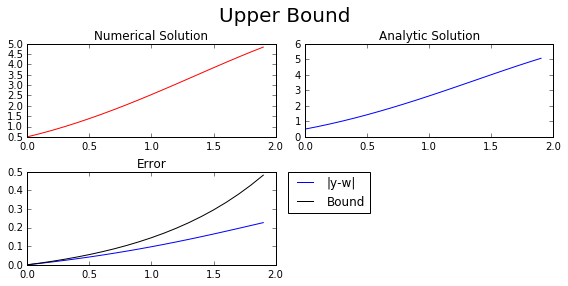
\includegraphics[scale=0.5]{UpperBound}
\caption{Python output: Illustrating upper bound $y^{'}=y-t^2+1$ with the initial condition $y(0)=0.5$ }
\label{UpperBound Figure}
\end{figure}
\end{example}
Euler method is a typical one step method, in general such methods are given by
function $\Phi(t,y;h;f)$. Our initial condition is $w_0=y_0$, for $i=0,1,..$
\[w_{i+1}=w_i+h\Phi(t_i,w_i:h:f)\]
with $t_{i+1}=t_i+h$.\\
In the Euler case $\Phi(t,y;h;f)=f(t,y)$ and is of order $1$.\\
Theorem \ref{Euler bound} can be extend to higher order one step methods with the variation 
\[ |y(t_i)-w_i| \leq \frac{Mh^p}{2L}|e^{L(t_i-a)}-1| \]
where $p$ is the order of the method.
\begin{definition}
The difference method $w_0=\alpha$
\[w_{i+1}=w_i+h\Phi(t_i,w_i),\]
for $i=0,1,...,N-1$ has a local truncation error given by
\begin{eqnarray*}
\tau_{i+1}(h) &=&\frac{y_{i+1}-(y_i+h\Phi(t_i,y_i))}{h},\\ 
&=&\frac{y_{i+1}-y_{i}}{h} -\Phi(t_i,y_i),
\end{eqnarray*}
for each $i=0,..,N-1$ where as usual $y_i=y(t_i)$ denotes the exact solution
at $t_i$.
\end{definition}
For Euler method the local truncation error at the ith step for the problem
\[ y^{'} = f(t,y), \ \ \ a\leq t \leq b, \ \ y(a)=\alpha, \]
is
\[\tau_{i+1}(h) =\frac{y_{i+1}-y_{i}}{h} -f(t_i,y_i), \]
for $i=0,..,N-1$.\\
But we know Euler has \[\tau_{i+1}=\frac{h}{2}y^{''}(\xi_i), \ \ \xi_i \in (t_i,t_{i+1}),\]
When $y^{''}(t)$ is known to be bounded by a constant M on $[a,b]$ this implies
\[|t_{i+1}(h)| \leq \frac{h}{2}M \sim O(h). \]
$O(h)$ indicates a linear order of error. The higher the order the more accurate the method.
\newpage
\section{Problem Sheet}
\begin{enumerate}
\item
Show that the following functions satisfy the Lipschitz condition on $y$ on the indicated set $D$:
\begin{enumerate}
\item
$f(t,y)=ty^3,$  $D=\{(t,y);-1\leq t \leq 1, 0\leq y \leq 10\};$
\item 
$f(t,y)=\frac{t^2y^2}{1+t^2},$  $D=\{(t,y);0\leq t, -10\leq y \leq 10 \}.$

\end{enumerate}
\item
Apply Euler's Method to approximate the solution of the given initial value problems using the indicated number of time steps. Compare the approximate solution with the given exact solution, and compare the actual error with the theoretical error
\begin{enumerate}
\item
$y'=t-y, \ \ (0\leq t \leq 4)$\\
with the initial condition $y(0)=1,$\\
$N=4$, 
$y(t)=2e^{-t}+t-1,$\\

The Lipschitz constant is determined on  $D=\{(t,y);0\leq t \leq 4, y\in \Re \}.$
\item 
$y'=y-t, \ \ (0\leq t \leq 2)$\\
with the initial condition $y(0)=2,$\\
$N=4$, 
$y(t)=e^{t}+t+1$.\\

The Lipschitz constant is determined on  $D=\{(t,y);0\leq t \leq 2, y\in \Re \}.$
\end{enumerate}

\end{enumerate}
\newpage
